%% abtex2-modelo-trabalho-academico.tex, v-1.9.6 laurocesar
%% Copyright 2012-2016 by abnTeX2 group at http://www.abntex.net.br/ 
%%
%% This work may be distributed and/or modified under the
%% conditions of the LaTeX Project Public License, either version 1.3
%% of this license or (at your option) any later version.
%% The latest version of this license is in
%%   http://www.latex-project.org/lppl.txt
%% and version 1.3 or later is part of all distributions of LaTeX
%% version 2005/12/01 or later.
%%
%% This work has the LPPL maintenance status `maintained'.
%% 
%% The Current Maintainer of this work is the abnTeX2 team, led
%% by Lauro César Araujo. Further information are available on 
%% http://www.abntex.net.br/
%%
%% This work consists of the files abntex2-modelo-trabalho-academico.tex,
%% abntex2-modelo-include-comandos and abntex2-modelo-references.bib
%%
% -------------------------------------------------------------------------
% -------------------------------------------------------------------------
%  abnTeX2: Modelo de Trabalho Academico (tese de doutorado, dissertacao de
%  mestrado e trabalhos monograficos em geral) em conformidade com 
%  ABNT NBR 14724:2011: Informacao e documentacao - Trabalhos academicos -
%  Apresentacao
% -------------------------------------------------------------------------
% -------------------------------------------------------------------------

\documentclass[
	% -- opções da classe memoir --
	12pt,				% tamanho da fonte
	openright,			% capítulos começam em pág ímpar (insere página vazia caso preciso)
	%twoside,			% para impressão em recto e verso. Oposto a oneside
	oneside,
	a4paper,			% tamanho do papel. 
	% -- opções da classe abntex2 --
	%chapter=TITLE,		% títulos de capítulos convertidos em letras maiúsculas
	%section=TITLE,		% títulos de seções convertidos em letras maiúsculas
	%subsection=TITLE,	% títulos de subseções convertidos em letras maiúsculas
	%subsubsection=TITLE,% títulos de subsubseções convertidos em letras maiúsculas
	% -- opções do pacote babel --
	english,			% idioma adicional para hifenização
	french,				% idioma adicional para hifenização
	spanish,			% idioma adicional para hifenização
	brazil				% o último idioma é o principal do documento
	]{abntex2}

% ---
% Pacotes básicos 
% ---
\usepackage{lmodern}			% Usa a fonte Latin Modern			
\usepackage[T1]{fontenc}		% Selecao de codigos de fonte.
\usepackage[utf8]{inputenc}		% Codificacao do documento (conversão automática dos acentos)
\usepackage{lastpage}			% Usado pela Ficha catalográfica
\usepackage{indentfirst}		% Indenta o primeiro parágrafo de cada seção.
\usepackage{color}				% Controle das cores
\usepackage{graphicx}			% Inclusão de gráficos
\usepackage{microtype} 			% para melhorias de justificação
\usepackage{multirow}
% ---
		
% ---
% Pacotes adicionais, usados apenas no âmbito do Modelo Canônico do abnteX2
% ---
\usepackage{lipsum}				% para geração de dummy text
% ---

% ---
% Pacotes de citações
% ---
\usepackage[brazilian,hyperpageref]{backref}	 % Paginas com as citações na bibl
\usepackage[alf]{abntex2cite}	% Citações padrão ABNT

% --- 
% CONFIGURAÇÕES DE PACOTES
% --- 

% ---
% Configurações do pacote backref
% Usado sem a opção hyperpageref de backref
\renewcommand{\backrefpagesname}{Citado na(s) página(s):~}
% Texto padrão antes do número das páginas
\renewcommand{\backref}{}
% Define os textos da citação
\renewcommand*{\backrefalt}[4]{
	\ifcase #1 %
		Nenhuma citação no texto.%
	\or
		Citado na página #2.%
	\else
		Citado #1 vezes nas páginas #2.%
	\fi}%
% ---

% ---
% Informações de dados para CAPA e FOLHA DE ROSTO
% ---
\titulo{Seleção dinâmica de interface em redes \\ IEEE 802.15.4}
\autor{Bruno Monteiro Pires}
\local{Rio Claro}
\data{2016}
\orientador{Alexandro José Baldassin}
\coorientador{Alex Roschildt Pinto}
\instituicao{
  Universidade Estadual Paulista -- UNESP
  \par
  Instituto de Biociências, Letras e Ciências Exatas
  \par
  Programa de Pós-Graduação em Ciência da Computação}
\tipotrabalho{Dissertação (Mestrado)}
% O preambulo deve conter o tipo do trabalho, o objetivo, 
% o nome da instituição e a área de concentração 

\preambulo{Dissertação de Mestrado elaborada junto ao Programa
	de Pós-Graduação em Ciência da Computação – Área
	de Concentração em Arquitetura de Computadores e
	Sistemas Distribuídos, como parte dos requisitos para
	obtenção do título de Mestre em Ciência da Computação.
}
% ---


% ---
% Configurações de aparência do PDF final

% alterando o aspecto da cor azul
\definecolor{blue}{RGB}{41,5,195}

% informações do PDF
\makeatletter
\hypersetup{
     	%pagebackref=true,
		pdftitle={\@title}, 
		pdfauthor={\@author},
    	pdfsubject={\imprimirpreambulo},
	    pdfcreator={LaTeX with abnTeX2},
		pdfkeywords={abnt}{latex}{abntex}{abntex2}{trabalho acadêmico}, 
		colorlinks=true,       		% false: boxed links; true: colored links
    	linkcolor=blue,          	% color of internal links
    	citecolor=blue,        		% color of links to bibliography
    	filecolor=magenta,      	% color of file links
		urlcolor=blue,
		bookmarksdepth=4
}
\makeatother
% --- 

% --- 
% Espaçamentos entre linhas e parágrafos 
% --- 

% O tamanho do parágrafo é dado por:
\setlength{\parindent}{1.3cm}

% Controle do espaçamento entre um parágrafo e outro:
\setlength{\parskip}{0.2cm}  % tente também \onelineskip

% ---
% compila o indice
% ---
\makeindex
% ---

% ---
% Set graphics path
% ---
\graphicspath{{images/}}

% ----
% Início do documento
% ----
\begin{document}

% Seleciona o idioma do documento (conforme pacotes do babel)
%\selectlanguage{english}
\selectlanguage{brazil}

% Retira espaço extra obsoleto entre as frases.
\frenchspacing 

% ----------------------------------------------------------
% ELEMENTOS PRÉ-TEXTUAIS
% ----------------------------------------------------------
% \pretextual

% ---
% Capa
% ---
\imprimircapa
% ---

% ---
% Folha de rosto
% (o * indica que haverá a ficha bibliográfica)
% ---
\imprimirfolhaderosto*
% ---

% ---
% Inserir a ficha bibliografica
% ---

% Isto é um exemplo de Ficha Catalográfica, ou ``Dados internacionais de
% catalogação-na-publicação''. Você pode utilizar este modelo como referência. 
% Porém, provavelmente a biblioteca da sua universidade lhe fornecerá um PDF
% com a ficha catalográfica definitiva após a defesa do trabalho. Quando estiver
% com o documento, salve-o como PDF no diretório do seu projeto e substitua todo
% o conteúdo de implementação deste arquivo pelo comando abaixo:
%
% \begin{fichacatalografica}
%     \includepdf{fig_ficha_catalografica.pdf}
% \end{fichacatalografica}

\begin{fichacatalografica}
	\sffamily
	\vspace*{\fill}					% Posição vertical
	\begin{center}					% Minipage Centralizado
	\fbox{\begin{minipage}[c][8cm]{13.5cm}		% Largura
	\small
	\imprimirautor
	%Sobrenome, Nome do autor
	
	\hspace{0.5cm} \imprimirtitulo  / \imprimirautor. --
	\imprimirlocal, \imprimirdata-
	
	\hspace{0.5cm} \pageref{LastPage} p. : il. (algumas color.) ; 30 cm.\\
	
	\hspace{0.5cm} \imprimirorientadorRotulo~\imprimirorientador\\
	
	\hspace{0.5cm}
	\parbox[t]{\textwidth}{\imprimirtipotrabalho~--~\imprimirinstituicao,
	\imprimirdata.}\\
	
	\hspace{0.5cm}
		1. IEEE802.15.4.
		I. Alexandro José Baldassin.
		II. Universidade Estadual Paulista.
		III. Instituto de Biociências, Letras e Ciências Exatas.
		IV. Seleção dinâmica de interface em redes IEEE 802.15.4
	\end{minipage}}
	\end{center}
\end{fichacatalografica}
% ---

% ---
% Inserir folha de aprovação
% ---

% Isto é um exemplo de Folha de aprovação, elemento obrigatório da NBR
% 14724/2011 (seção 4.2.1.3). Você pode utilizar este modelo até a aprovação
% do trabalho. Após isso, substitua todo o conteúdo deste arquivo por uma
% imagem da página assinada pela banca com o comando abaixo:
%
% \includepdf{folhadeaprovacao_final.pdf}
%
\begin{folhadeaprovacao}

  \begin{center}
    {\ABNTEXchapterfont\large\imprimirautor}

    \vspace*{\fill}\vspace*{\fill}
    \begin{center}
      \ABNTEXchapterfont\bfseries\Large\imprimirtitulo
    \end{center}
    \vspace*{\fill}
    
    \hspace{.45\textwidth}
    \begin{minipage}{.5\textwidth}
        \imprimirpreambulo
    \end{minipage}%
    \vspace*{\fill}
   \end{center}
        
   Trabalho aprovado. \imprimirlocal, 22 de dezembro de 2016:

   \assinatura{\textbf{\imprimirorientador} \\ Orientador} 
   \assinatura{\textbf{Professor} \\ Convidado 1}
   \assinatura{\textbf{Professor} \\ Convidado 2}
   %\assinatura{\textbf{Professor} \\ Convidado 3}
   %\assinatura{\textbf{Professor} \\ Convidado 4}
      
   \begin{center}
    \vspace*{0.5cm}
    {\large\imprimirlocal}
    \par
    {\large\imprimirdata}
    \vspace*{1cm}
  \end{center}
  
\end{folhadeaprovacao}
% ---

% ---
% Dedicatória
% ---
\begin{dedicatoria}
   \vspace*{\fill}
   \centering
   \noindent
   \textit{ Este trabalho é dedicado às crianças adultas que,\\
   quando pequenas, sonharam em se tornar cientistas.} \vspace*{\fill}
\end{dedicatoria}
% ---

% ---
% Agradecimentos
% ---
\begin{agradecimentos}
Os agradecimentos principais são direcionados à Gerald Weber, Miguel Frasson,
Leslie H. Watter, Bruno Parente Lima, Flávio de Vasconcellos Corrêa, Otavio Real
Salvador, Renato Machnievscz\footnote{Os nomes dos integrantes do primeiro
projeto abn\TeX\ foram extraídos de
\url{http://codigolivre.org.br/projects/abntex/}} e todos aqueles que
contribuíram para que a produção de trabalhos acadêmicos conforme
as normas ABNT com \LaTeX\ fosse possível.

Agradecimentos especiais são direcionados ao Centro de Pesquisa em Arquitetura
da Informação\footnote{\url{http://www.cpai.unb.br/}} da Universidade de
Brasília (CPAI), ao grupo de usuários
\emph{latex-br}\footnote{\url{http://groups.google.com/group/latex-br}} e aos
novos voluntários do grupo
\emph{\abnTeX}\footnote{\url{http://groups.google.com/group/abntex2} e
\url{http://www.abntex.net.br/}}~que contribuíram e que ainda
contribuirão para a evolução do \abnTeX.

\end{agradecimentos}
% ---

% ---
% RESUMOS
% ---

% resumo em português
%\setlength{\absparsep}{18pt} % ajusta o espaçamento dos parágrafos do resumo
%\begin{resumo}
% Segundo a \citeonline[3.1-3.2]{NBR6028:2003}, o resumo deve ressaltar o
% objetivo, o método, os resultados e as conclusões do documento. A ordem e a extensão
% destes itens dependem do tipo de resumo (informativo ou indicativo) e do
% tratamento que cada item recebe no documento original. O resumo deve ser
% precedido da referência do documento, com exceção do resumo inserido no
% próprio documento. (\ldots) As palavras-chave devem figurar logo abaixo do
% resumo, antecedidas da expressão Palavras-chave:, separadas entre si por
% ponto e finalizadas também por ponto.

% \textbf{Palavras-chave}: latex. abntex. editoração de texto.
%\end{resumo}

% resumo em inglês
%\begin{resumo}[Abstract]
% \begin{otherlanguage*}{english}
%   This is the english abstract.

%   \vspace{\onelineskip}
 
%   \noindent 
%   \textbf{Keywords}: latex. abntex. text editoration.
% \end{otherlanguage*}
%\end{resumo}
% ---

% ---
% inserir lista de ilustrações
% ---
\pdfbookmark[0]{\listfigurename}{lof}
\listoffigures*
\cleardoublepage
% ---

% ---
% inserir lista de tabelas
% ---
\pdfbookmark[0]{\listtablename}{lot}
\listoftables*
\cleardoublepage
% ---

% ---
% inserir lista de abreviaturas e siglas
% ---
%\begin{siglas}
%  \item[ABNT] Associação Brasileira de Normas Técnicas
%  \item[abnTeX] ABsurdas Normas para TeX
%\end{siglas}
% ---

% ---
% inserir lista de símbolos
% ---
%\begin{simbolos}
%  \item[$ \Gamma $] Letra grega Gama
%  \item[$ \Lambda $] Lambda
%  \item[$ \zeta $] Letra grega minúscula zeta
%  \item[$ \in $] Pertence
%\end{simbolos}
% ---

% ---
% inserir o sumario
% ---
\pdfbookmark[0]{\contentsname}{toc}
\tableofcontents*
\cleardoublepage
% ---



% ----------------------------------------------------------
% ELEMENTOS TEXTUAIS
% ----------------------------------------------------------
\textual

% ----------------------------------------------------------
% Introdução
% ----------------------------------------------------------
\chapter[Introdução]{Introdução}
Redes de sensores sem fios têm, desde seu surgimento, possibilitado o monitoramento dos mais diversos fenômenos e processos, além de abrir caminho para a criação de uma nova geração de sistemas inteligentes, dinâmicos e conectados. Historicamente esforços visionários como Igloo White \cite{Warneke2001} e Smart Dust \cite{Correl2004} demonstraram o potencial desta tecnologia. No entanto, até o momento, são raras as iniciativas realizadas no sentido de idealizar plataformas de uso geral.

A diversidade das aplicações as quais se destinam as redes de sensores sem fios impõe restrições no projeto e na implantação destes sistemas, o que favorece iniciativas de desenvolvimento orientadas à aplicação. Embora esta abordagem leve à criação de soluções eficazes para aplicações específicas, estabelece um padrão de desenvolvimento restrito e desconsidera possibilidades de otimização mais abrangentes. Além de inibir eventuais reduções de custo resultantes da produção em massa e difusão da tecnologia \cite{Rawat2014}. 

É possível supor que dentre as motivações para adoção generalizada deste modelo de desenvolvimento esteja o fato de as pesquisas na área terem se iniciado antes que as tecnologias que as viabilizam estivessem totalmente desenvolvidas. Tal consideração fica evidente quando se observa, por exemplo, a história de Igloo White. Uma operação militar responsável por monitorar os campos de batalha durante a guerra do Vietnã, através do que talvez tenha sido a primeira utilização documentada de uma rede de sensores sem fios. Na época foi necessário que cada um de seus componentes fosse projetado sob medida, assim como a infraestrutura necessária para coleta e posterior processamento dos dados obtidos. Isso fez com que a operação demandasse uma quantidade exorbitante de recursos, sendo sua execução assegurada somente após substanciais investimentos do departamento de defesa dos Estados Unidos.

Efetivamente diversas das motivações para que se desenvolvessem redes de sensores sem fios e sistemas de informação similares já existiam muito antes que as tecnologias disponíveis possibilitassem a implementação de soluções viáveis. Por este motivo a área sempre foi muito beneficiada pelos avanços realizados no campo da microeletrônica de baixa potência, que vêm acontecendo de forma regular. Isso faz com que frequentemente barreiras técnicas sejam superadas, alterando paradigmas de projeto e abrindo caminho para exploração de novos mercados e aplicações. Razão pela qual o tema continua recebendo tanta atenção, apesar de as pesquisas na área terem começado a se intensificar já no início dos anos 2000 \cite{Kahn2000, Pottie2000, Heinzelman2000}, quase duas décadas atrás.

Contudo o maior motivador para o crescente interesse no desenvolvimento de redes de sensores sem fios foi, sem dúvida, o surgimento do conceito de Internet das Coisas, ou \textit{Internet of Things} (IoT). Um paradigma tecnológico no qual se propõe que os mais diversos objetos devam ser equipados de forma a permitir que se comuniquem, diretamente e através da Internet, e que possam ser acessados remotamente a fim de prover informações úteis, ou ainda, realizar ações. Segundo \cite{Harrop2014}, os mercados relacionados às redes de sensores sem fios devem chegar a movimentar cerca de 1.8 bilhões de dólares até 2024, sendo esta soma referente somente aos sistemas de rede com topologia \textit{mesh}. Estima-se também um crescimento exponencial na quantidade de dispositivos conectados, podendo esta atingir um total de 25 bilhões de dispositivos até 2020 \cite{Want2015}. Para que esta demanda possa ser atendida, no entanto, ainda existem diversos desafios a serem superados. Se destacam questões como padronização dos protocolos de comunicação e interoperabilidade \cite{Rawat2014, IEC2014}, dentre outros tópicos vinculados à massificação desta tecnologia. 

Neste âmbito a obtenção de links de comunicação versáteis e confiáveis é essencial, sendo que o método mais disseminado atualmente é a transmissão de dados via radiofrequência. Se comparada a outras técnicas, a utilização de radiotransmissores oferece maior flexibilidade quanto à topologia das redes e simplifica o processo de implantação, pois permite que se integrem novos dispositivos à infraestrutura já existente sem que sejam necessárias grandes intervenções.

No entanto a qualidade dos links de rádio sofre influencia de diversas variáveis externas como, por exemplo: interferência gerada por outros equipamentos, alterações na vegetação, objetos se movendo nas proximidades e até mesmo mudanças nas condições climáticas. Logo a eficiência destes links tende a variar ao longo do tempo e de acordo com a localização dos transmissores \cite{Kusy2011}. Protocolos de roteamento modernos são capazes de lidar com estas adversidades detectando alterações na qualidade dos links individuais e estabelecendo rotas alternativas a fim de otimizar o fluxo de dados na rede e garantir maior eficiência energética \cite{Gnawali2009}. No entanto esta abordagem depende do provisionamento de rotas alternativas, requerendo redes mais densas, o que eleva os custos e pode dificultar o processo de implantação.

\section{Objetivos e Contribuições}
Este trabalho tem como objetivo principal explorar alternativas para mitigar os problemas de instabilidade relacionados aos links de rádio nas redes de sensores sem fios. Diversas iniciativas já foram realizadas com este intuito, contudo se trata de um espaço de soluções bastante amplo e diversificado, havendo ainda grande potencial para otimização. A abordagem proposta nas seções seguintes buscará utilizar mais intensivamente o hardware e as camadas inferiores dos protocolos de comunicação, a fim de permitir a implementação de plataformas mais flexíveis e robustas, capazes de operar em uma maior gama de situações. 

A fim de validar estas propostas experimentalmente será introduzida, na seção \ref{phynode}, a plataforma PhyNode. A abordagem utilizada em sua construção tem o potencial de contribuir para o estado da arte das pesquisas na área, pois complementa outras soluções já presentes na literatura \cite{Pantazis2013, Tarique2009} e que, em grande parte, são destinadas exclusivamente a ambientes de rede \textit{mesh} densamente populados e redundantes, além de não dedicarem atenção especial às possibilidades proporcionadas pela utilização de hardware especificamente destinado à manutenção de links de comunicação mais robustos.

É interessante que soluções como PhyNode sejam desenvolvidas com o objetivo de incentivar o processo de massificação do uso de sistemas baseados em redes de sensores sem fios. A medida que esta tecnologia é integrada a um número maior de produtos e disponibilizada aos consumidores finais, se torna essencial que seja capaz de operar de forma confiável em diferentes ambientes e através de topologias bastante diversificadas. Atualmente a maior parte das redes de sensores sem fios é utilizada em pesquisas científicas, com fins exploratórios, permitindo que cada projeto seja realizado considerando ambientes de aplicação específicos. Este paradigma, no entanto, não é adequado para as aplicações comerciais, onde a produção em massa se beneficia de projetos mais flexíveis, que possibilitem a produção em larga escala e sejam capazes de adaptar-se a diferentes aplicações.

\section{Organização do texto}
% TODO - Organização do texto
% ---

% ---
% Fundamentação teórica e trabalhos relacionados
% ---
\chapter{Fundamentação teórica}
A fim de embasar as discussões apresentadas ao longo deste trabalho, esta seção será dedicada a apresentar os diversos conceitos que serão futuramente utilizados, começando pela própria arquitetura associada às redes de sensores sem fios. Estes sistemas são definidos como redes compostas por um conjunto de nodos de sensores (também conhecidos como \textit{motes}), capazes de estabelecer uma infraestrutura de comunicação de forma \textit{ad-hoc}, e utiliza-la para coletar e transmitir dados obtidos a partir dos sensores presentes em cada nodo. Podem contar ainda com um ou mais \textit{sinks}, responsáveis por concentrar a coleta dos dados obtidos, e \textit{gateways}, responsáveis por fazer a ponte entre os nodos que compõem a rede e o exterior, disponibilizando os dados coletados a uma rede local ou transmitindo-os diretamente para a internet. A arquitetura ilustrada na \autoref{fig_node_generic} será considerada daqui em diante como o modelo básico de um nodo de sensores sem fio. 

\begin{figure}[htb]
	\caption{\label{fig_node_generic}Nodo de sensores sem fio: arquitetura básica}
	\begin{center}
		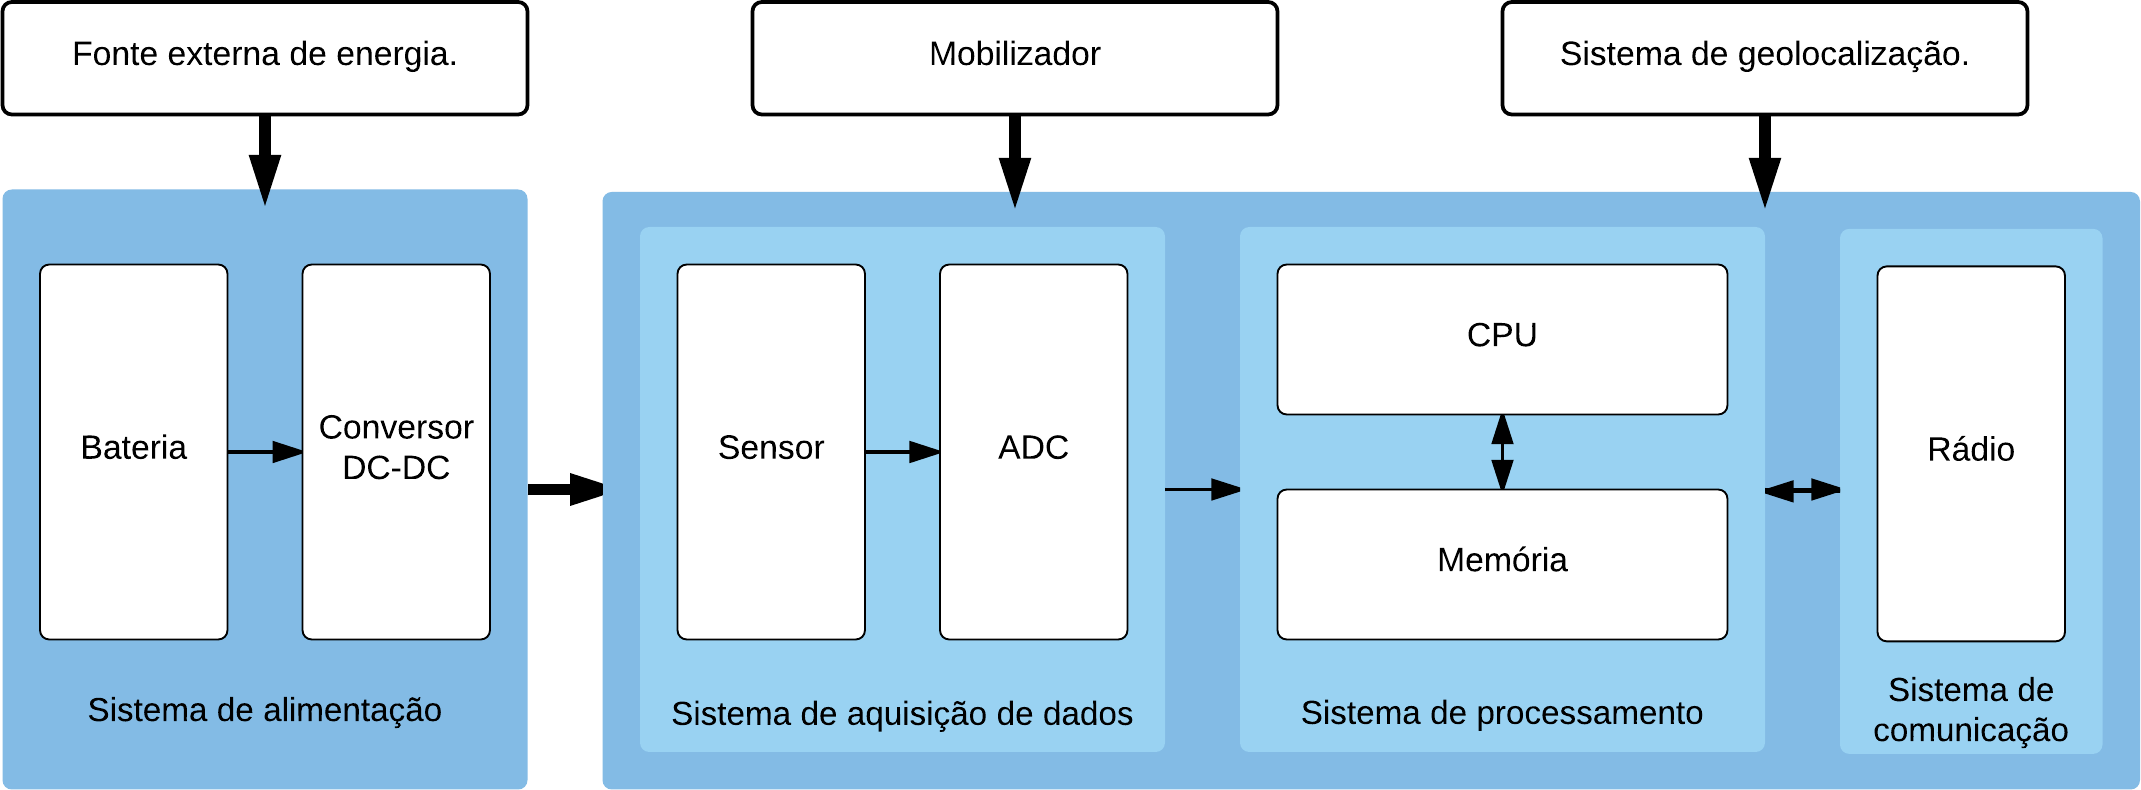
\includegraphics[width=\linewidth]{SensorNode_Generic}
	\end{center}
	\legend{Adaptado de \citeonline{Anastasi2009}}
\end{figure}

Cada nodo de sensor representado por esta arquitetura é composto essencialmente por quatro subsistemas \cite{Akyildiz2002, Rawat2014}.

\begin{itemize}
	\item \textit{Sistema de alimentação.} Responsável pelo fornecimento de energia aos demais componentes, deve realizar a regulação de voltagem e outras adequações que se façam necessárias nas linhas de alimentação do nodo. Pode ainda realizar a captura e o armazenamento da energia proveniente de fontes secundárias, quando disponíveis. É essencialmente composto por uma ou mais baterias primárias e um conversor DC-DC, capaz de manter, de forma eficiente, os níveis de voltagem adequados nas linhas de alimentação.
	\item \textit{Sistema de aquisição de dados.} É capaz de obter dados amostrais a partir dos fenômenos monitorados, quando solicitado. Deve contar com um ou mais transdutores, responsáveis por converter as grandezas físicas monitoradas em sinais elétricos analógicos. E com circuitos de conversão analógico-digital (ADC's), cujo propósito é realizar a conversão dos sinais analógicos, provenientes dos transdutores, em sinais digitais compatíveis com as interfaces do sistema de processamento.
	\item \textit{Sistema de processamento.} É responsável por coordenar as tarefas delegadas ao nodo como, por exemplo, a obtenção de dados amostrais ou o roteamento de pacotes de dados encaminhados por outros nodos. Este sistema é composto essencialmente de um microcontrolador com memória integrada e, opcionalmente, pode contar com módulos de memória adicionais, a fim de permitir o armazenamento de maiores quantidades de dados localmente. O que pode vir a ser necessário de acordo com a topologia da rede ou caso não haja disponibilidade de conexões com o exterior.
	\item \textit{Sistema de comunicação.} É o responsável por permitir que os dados trafeguem entre os nodos que compõem a rede. Sua implementação mais comum, e a que será considerada ao longo deste trabalho, se baseia na utilização de radiotransmissores de baixa potência. No entanto vale ressaltar que as possibilidades de implementação não se restringem somente a este método. Em casos específicos, e onde a transmissão via rádio não é vantajosa, factível ou financeiramente viável, outros métodos de comunicação, como infra-vermelho ou transmissores acústicos, podem ser utilizados.
\end{itemize}

Algumas aplicações podem ainda requerer sistemas adicionais, como, por exemplo: sistemas de geolocalização (capazes de determinar a localização geográfica de determinado nodo); sistemas de mobilização (capazes de mover os nodos equipados entre diferentes posições, ou ainda, de reorientar antenas direcionais); sistemas de localização relativa (capazes de determinar a posição de um nodo em relação aos demais). A implementação destes sistemas pode tanto requerer hardware adicional ou permitir que sejam implementados puramente em software. No entanto, por se tratarem de componentes raramente utilizados, não serão considerados parte integrante do modelo básico, definido anteriormente.

Existem ainda os \textit{gateways} e \textit{sinks}, cuja arquitetura básica se assemelha à presente nos demais nodos. No entanto \textit{gateways} devem contar com interfaces de comunicação secundárias, capazes de estabelecer conexão entre a rede de sensores e alguma rede externa, ou diretamente com a internet. Já os \textit{sinks}, devem ser capazes de armazenar maior quantidade de dados localmente. Ambos frequentemente possuem maior poder de processamento, a fim de permitir que lidem com a carga extra de trabalho sem criar gargalos. Geralmente as funções de \textit{sink} e \textit{gateway} são atribuídas aos mesmos nodos, facilitando a coleta ou transferência dos dados coletados.

Para melhor compreender os desafios com os quais as propostas realizadas nas seções \ref{phynode} e \ref{phymac} visam lidar, certos aspectos específicos da operação dos nodos devem ser esclarecidos. A seguir serão melhor discutidas algumas peculiaridades e métodos relacionados à conservação de energia, protocolos de roteamento e estimativa de qualidade dos links de rádio, nas redes de sensores sem fios. Serão também analisadas iniciativas realizadas no sentido de fornecer padrões de implementação e operação.

\section{Conservação de energia}
A distribuição do consumo energético dentre os diferentes subsistemas, bem como as rotinas empregadas para transmissão e aquisição de dados, estão parcialmente sujeitas aos requisitos específicos das aplicações. No entanto algumas observações gerais são aplicáveis à maioria dos sistemas \cite{Anastasi2009}.

\begin{itemize}
	\item O consumo apresentado pelos sistemas de comunicação é muito superior ao originado no sistema de processamento. Sendo a energia utilizada para transmitir um único bit via rádio equivalente à empregada no processamento de até mil instruções, num nodo típico \cite{Pottie2000}. Sendo assim, é mais vantajoso aplicar processamento local, a fim de reduzir o volume de dados a ser transmitido, do que transmitir grandes quantidades de dados brutos.
	\item O consumo energético apresentado pelos transmissores de rádio nos modos de recepção, transmissão e espera é da mesma ordem. Existem, no entanto, em grande parte dos transmissores atuais, modos de baixo consumo, cuja utilização geralmente resulta em certa latência adicional, porém devem ser utilizados sempre que os protocolos de rede permitirem.
	\item O consumo do sistema de aquisição de dados é altamente dependente dos requisitos da aplicação, sendo em muitos casos significativo, e até mesmo superior ao consumo do sistema de comunicação. Nestes casos, torna-se interessante utilizar algoritmos destinados especificamente a minimizar o consumo referente à coleta de dados.
\end{itemize}

\begin{figure}[htb]
	\caption{\label{fig_energy_conservation}Técnicas para conservação de energia}
	\begin{center}
		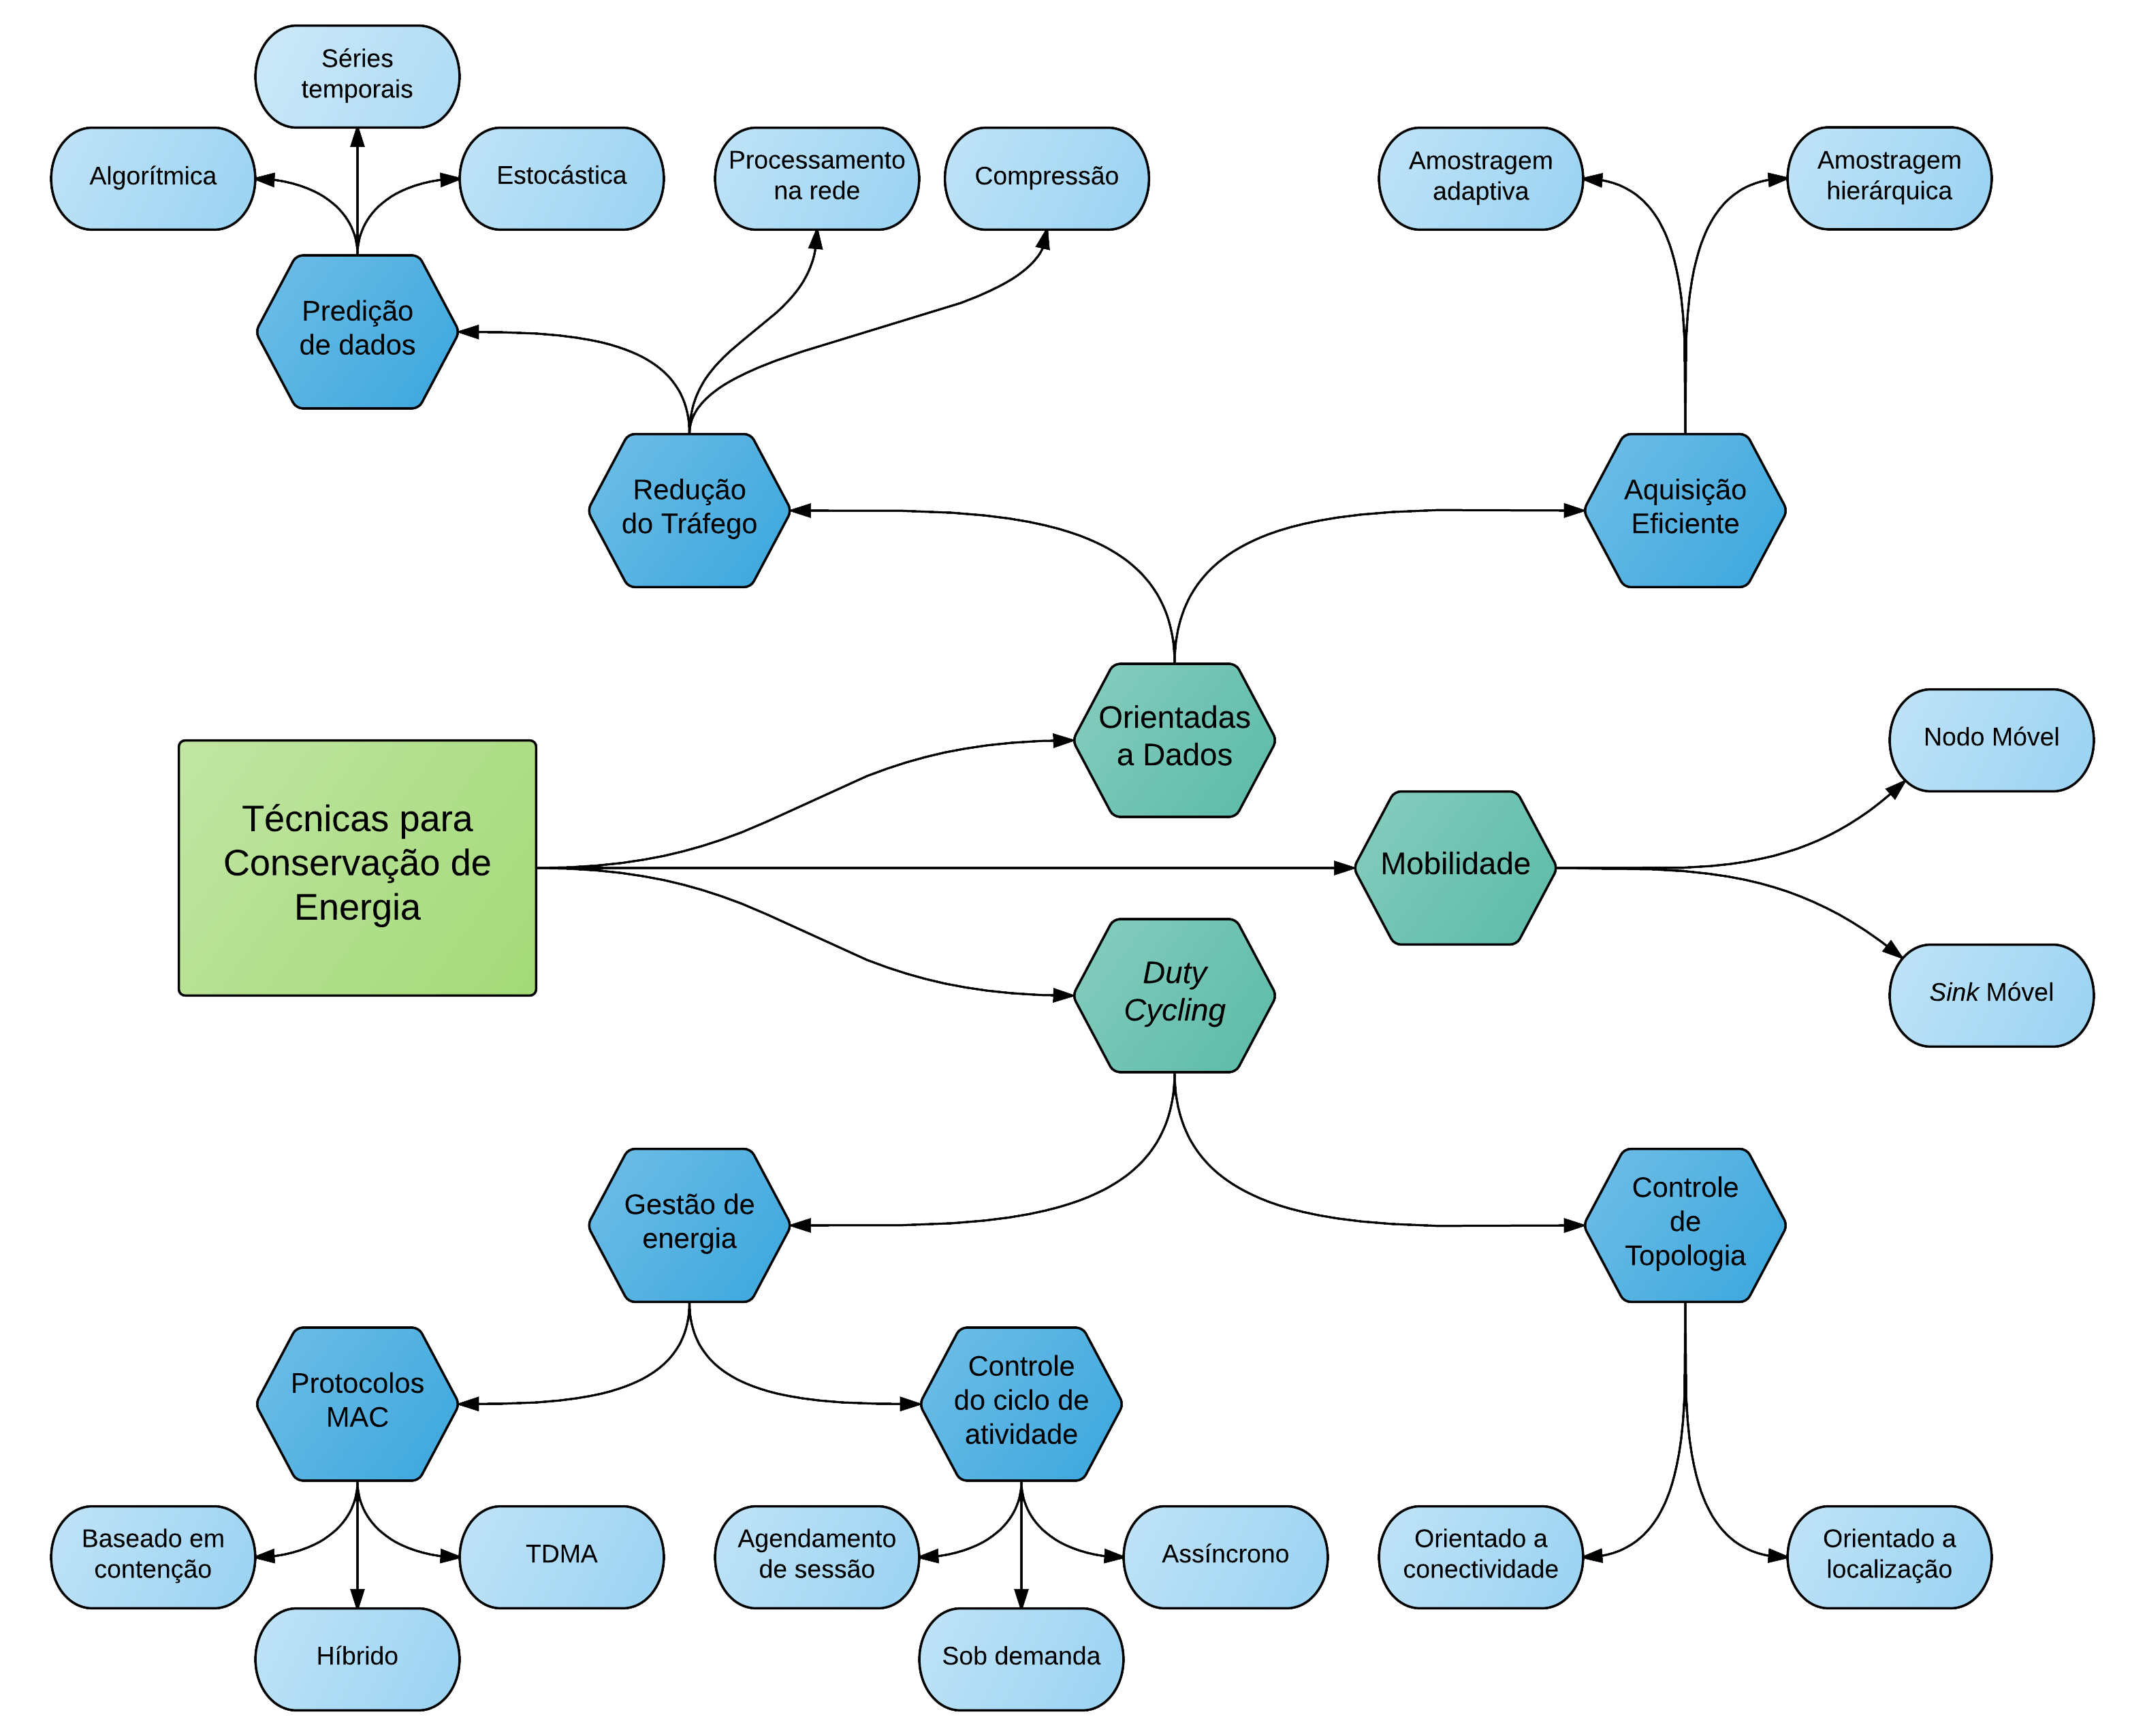
\includegraphics[width=\linewidth]{EnergyConservation}
	\end{center}
	\legend{Adaptado de \citeonline{Anastasi2009}}
\end{figure}

Baseando-se nestas premissas é possível explorar diversas abordagens para otimizar o consumo de energia nos nodos de sensor. A \autoref{fig_energy_conservation} apresenta uma classificação hierárquica destas técnicas, como proposta em \cite{Anastasi2009}. Embora mais de uma dezena de técnicas específicas sejam apresentadas, conceitualmente estas abordagens podem ser todas classificadas em três subcategorias principais: técnicas baseadas em \textit{duty-cycling}, técnicas orientadas a dados e técnicas orientadas a mobilidade.

\subsection{Técnicas baseadas em \textit{duty-cycling}}

Técnicas baseadas em \textit{duty-cycling} consistem em estabelecer estratégias para que determinados sistemas dos nodos possam, periodicamente, ser desativados ou colocados em estados de baixo consumo. Possibilitam desta maneira que haja uma redução na média do consumo energético proveniente do sistema em questão. O período de atividade, ou \textit{duty-cycle}, é um valor percentual que representa a fração de tempo durante a qual este subsistema deverá manter-se ativo dentro de um determinado período de tempo.

Embora também possam ser aplicadas aos demais sistemas, técnicas desta natureza são comumente utilizadas para o controle do sistema de comunicação, dado que neste caso podem proporcionar melhorias significativas devido ao alto consumo deste sistema. Contudo o aumento na latência dos links de comunicação, ocasionado pela indisponibilidade dos transceptores durante os períodos em que são colocados em modos de baixo consumo, faz com que esta abordagem não seja adequada em todas as situações. Convenientemente em alguns casos é possível variar o \textit{duty-cycle} dinamicamente, de acordo com a intensidade do tráfego, por exemplo, a fim de proporcionar um melhor comprometimento entre a redução do consumo de energia e a latência dos links de comunicação.

\subsection{Técnicas orientadas a dados}

Apesar de as técnicas baseadas em \textit{duty-cycling} permitirem certa conservação de energia ao impedir que certos sistemas do nodo permaneçam em modos de alto consumo durante períodos de inatividade, por definição elas não dispõem dos meios para análise dos dados coletados pelo sensores ou retransmitidos. Assim sendo, ignoram quaisquer redundâncias presentes nas informações que circulam pela rede, potencialmente permitindo que alguma energia seja desperdiçada durante a manipulação de dados essencialmente desnecessários. Já as técnicas orientadas a dados são especificamente destinadas a analisar estes dados, de forma a eliminar possíveis redundâncias e evitar ciclos de amostragem ou retransmissões desnecessárias. Estas técnicas operam na camada de aplicação, sendo geralmente utilizadas em conjunto com outros métodos, operando em camadas inferiores, a fim de reduzir ainda mais o consumo energético das redes de sensores.

Mais especificamente, a ausência de métodos destinados ao controle de redundâncias afeta a eficiência energética da rede permitindo que dois tipos distintos de evento ocorram:

\begin{itemize}
	\item \textit{Transmissão de dados redundantes.} Dados amostrais geralmente apresentam forte correlação espacial e temporal logo, para satisfazer os requisitos de determinadas aplicações, pode não ser necessário transmitir na íntegra todas as amostras coletadas. É possível ainda aplicar técnicas de agregação e compressão de dados a fim de reduzir o volume de tráfego sem omitir amostras já coletadas.
	\item \textit{Aquisição de dados redundantes.} Alguns sistemas de aquisição apresentam alto consumo de energia, nestes casos o ideal é evitar, sempre que possível, que sejam realizados ciclos de amostragem desnecessários. Para tal geralmente são empregados algoritmos especializados, responsáveis por verificar se dados equivalentes foram previamente coletados (localmente ou por nodos próximos) antes que se iniciem novas amostragens.
\end{itemize}

\subsection{Técnicas orientadas à mobilidade}

Existem ainda técnicas de conservação de energia baseadas na mobilidade de nodos. Durante sua operação de rotina, os nodos de uma rede de sensores sem fios conduzem os dados coletados em direção aos \textit{sinks}. A principal consequência deste paradigma é a sobrecarga dos meios de transmissão dos nodos localizados próximo aos \textit{sinks}, através dos quais deverão ser roteados na íntegra os dados coletados pela rede \cite{Li2007}. A sobrecarga dos meios de transmissão nesta região provoca um consumo acelerado das reservas de energia dos nodos envolvidos: em geral os protocolos de comunicação se tornam menos eficientes em regiões sobrecarregadas, devido à possibilidade de ocorrerem colisões e, consequentemente, tentativas de retransmissão. A exaustão prematura das fontes de energia destes nodos, por sua vez, pode levar à subutilização de nodos mais distantes que, apesar de não terem suas reservas energéticas esgotadas, são inutilizados caso deixem de dispor de rotas de acesso aos \textit{sinks}.

Neste contexto, nodos ou \textit{sinks} móveis podem ser utilizados a fim de mitigar a sobrecarga de certas regiões, realizando a coleta dos dados enquanto se movimentam através da rede. Esta abordagem exige que os nodos estáticos fiquem à espera da passagem dos nodos móveis, quando terão a oportunidade de transmitir os dados diretamente a um \textit{sink} móvel, ou através de rotas mais eficientes. Este processo beneficia po balanceamento de cargas e possibilita a utilização uniforme das reservas de energia de todos os nodos estáticos. Ao eliminar regiões potencialmente sobrecarregadas é possível ainda obter algum aumento na eficiência dos protocolos de comunicação, devido à redução dos níveis de contenção (tentativas frustradas de acesso aos meios de transmissão). Para que estas abordagens sejam efetivas, no entanto, deve-se planejar cuidadosamente os padrões de movimentação dos nodos móveis. Caso se torne muito complexo ou dispendioso projetar nodos móveis customizados, existe ainda a possibilidade de utilizar-se de entidades que já se movimentem pela área monitorada, como veículos ou animais.

\section{Estimativa de qualidade  dos links}

A propagação dos sinais de rádio, principalmente nos links de baixa potência como os utilizados nas redes de sensores sem fios, é significativamente afetada por diversos fatores externos que contribuem para sua degradação. O que faz com que estes links se comportem de forma errática, sendo que sua performance pode variar ao longo do tempo, e de acordo com a localização dos nodos. Falhas de transmissão, como o corrompimento ou perda dos pacotes de dados e as ações subsequentes, destinadas à correção destas falhas, chegam a ser responsáveis por 50\% a 80\% do consumo de energia proveniente dos sistemas de comunicação, variando de acordo com a intensidade do tráfego \cite{Srinivasan2006}. Além de prejudicar a execução de protocolos de mais alto nível, uma vez que a largura de banda disponível é efetivamente reduzida e inviabiliza-se transações que imponham restrições temporais rigorosas.

As perturbações responsáveis por degradar a qualidade dos links são causadas por fenômenos cujo comportamento e origens são bastante distintos. No entanto podem ser classificadas quanto à sua natureza em duas principais categorias: atenuação e interferência. Entende-se por atenuação a absorção ou reflexão parcial, em decorrência da interação com o ambiente, dos sinais de rádio emitidos por um transmissor. O que resulta numa redução da intensidade do sinal captado pelo receptor. Já o termo interferência se refere ao acoplamento de sinais externos, e de frequência similar, às transmissões realizada entre um transmissor e um receptor. Este processo causa distorções no sinal original e resulta no corrompimento dos dados transmitidos sem que haja, necessariamente, qualquer redução na intensidade do sinal captado pelo receptor. De acordo com \cite{Baccour2012} são três os principais fatores que exercem influência sobre a qualidade dos links de rádio:
\begin{itemize}
	\item \textit{O ambiente.} Além de ser o principal componente para a atenuação dos sinais, também é responsável pela ocorrência do fenômeno conhecido como propagação multicaminho: quando, ao se propagar através de certo ambiente, componentes parciais de um mesmo sinal são refletidos e dispersam-se através de múltiplas rotas, cada um deles atingindo o receptor com diferentes intensidades e ligeira defasagem temporal \cite{Kusy2011}. O que resulta na distorção do sinal original e leva ao corrompimento dos dados. O ambiente também determina os níveis de ruído de fundo, contribuindo para determinação da relação entre sinal e ruído.
	\item \textit{O hardware.} O hardware dos transmissores invariavelmente apresenta alguma variabilidade, devido a seu próprio ruído interno e às faixas de tolerância aplicadas aos valores dos componentes utilizados para sua construção \cite{Goldsmith2005}. Com o desenvolvimento de hardware mais atualizado, este fator tende a exercer menor influência na qualidade final dos links, porém não deve ser desconsiderado durante a concepção de métodos de estimativa de qualidade ou protocolos de comunicação. 
	\item \textit{Interferência de sinais externos.} É causada pela presença de múltiplos sinais sendo transmitidos concorrentemente, num mesmo ambiente, através de faixas de frequência similares. Podendo estes sinais originarem-se em diferentes nodos de uma mesma rede de sensores, outros equipamentos que compartilhem a mesmas faixas de frequência para comunicação sem fios, ou ainda resultado de ruído eletromagnético gerado involuntariamente por certos equipamentos elétricos.
\end{itemize}



\section{Iniciativas de padronização}
A norma IEEE 802.15.4 \cite{IEEE2003}, define um protocolo de comunicação e parâmetros de implementação da camada física para interconexão de dispositivos via radiofrequência em redes de área pessoal sem fio com baixas taxas de transmissão (LR-WPANs). Esta norma é base para alguns dos protocolos mais disseminados na indústria como ZigBee \cite{bibid}, 6LowPAN \cite{bibid}, WirelessHART \cite{bibid}, MiWi \cite{bibid} entre outros. A norma original, publicada em 2003, propunha apenas duas implementações distintas para a camada física (PHY), sendo a primeira destinada à operação nas bandas de 868 MHz e 915 MHz utilizando modulação BPSK e a segunda na banda de 2450 MHz, através da modulação O-QPSK. Desde sua publicação original, no entanto, esta norma recebeu diversas emendas e revisões, através das quais foram adicionados novos PHYs e realizadas alterações nos protocolos de comunicação. 

Dispositivos compatíveis devem implementar por completo ao menos um PHY, podendo opcionalmente ser compatíveis com múltiplos PHYs. A seleção dos PHYs a serem utilizados, no entanto, fica a cargo das regulamentações locais e preferências do usuário. Em sua última versão, IEEE 802.15.4-2015 \cite{IEEE2016}, há dezenove PHYs, capazes de operar em bandas de frequência que variam entre 169 MHz e cerca de 9 GHz. A grande diversidade de  implementações prevista pela norma faz com que frequentemente as legislações vigentes em cada país sejam compatíveis, simultaneamente, com diversas delas.
 % ---
Cada PHY define uma modulação específica, taxas de transferência distintas e um certo número de canais para cada banda de frequência suportada. Sendo que cada canal representa uma pequena faixa de frequência dentro do espectro da banda a qual pertence. A quantidade de canais disponíveis em cada PHY pode variar, de acordo com a largura de banda dedicada a cada um deles. 

A seleção do método de acesso ao meio físico na norma IEEE 802.15.4 é realizada através de um identificador único de 32 bits, composto por um número de página (armazenado nos 5 bits mais altos) e um número de canal (27 bits restantes). Esta arquitetura foi introduzida com o intuito de permitir a declaração de novos PHYs a medida que fossem realizadas novas revisões do protocolo. 

\section{Discussão}
Motes are equipped with a low-rate (10–100 kbps) and short-range (less than 100 m) wireless radio, e.g., IEEE 802.15.4 radio to communicate among themselves. 
Since radio communication consumes most of the power, the radio must incorporate energy-efficient communication techniques.
The power source commonly used is rechargeable batteries.
Since motes can be deployed in remote and hostile environments they must use little power and must employ built-in mechanisms to extend network lifetime.
For example, motes may be equipped with effective power harvesting methods, such as solar cells, so they may be left unattended for years \cite{Rawat2014}.

Devido às restrições na complexidade, no consumo energético e nos custos de produção, os transmissores de rádio utilizados para este fim geralmente operam com baixa potência e pequenas taxas de transmissão. Isso faz com que os links estabelecidos se tornem bastante susceptíveis à variações intermitentes de qualidade, especialmente nos casos em que compartilham sua banda de frequência com outros sistemas mais bem difundidos. Como é o caso da disputada faixa de 2.4GHz, na qual também estão outras tecnologias bem difundidas como WiFi e Bluetooth.


\chapter{Trabalhos relacionados}
	\section{Diversidade de interfaces}
	\section{Estimativa de qualidade dos links}
	\section{Discussão}
% ---

% ---
% Materiais e Métodos
% ---
\chapter{PhyNode: plataforma de desenvolvimento} \label{phynode}

Dado que a utilização de diferentes modulações, ou bandas de frequência, resulta, de acordo com as condições do ambiente, em alterações na qualidade dos links de rádio \cite{bibid}, considera-se que seja possível explorar a diversificação de interfaces admitida pela norma a fim de otimizar a performance de links de comunicação. No caso de dispositivos dotados de múltiplas interfaces, uma forma através da qual este objetivo pode ser alcançado é utilizando um algoritmo de seleção dinâmica, capaz de eleger a interface mais adequada, a cada momento, para a transferência dos dados. Com este objetivo, nas seções seguintes, será proposta a arquitetura batizada de PhyNode, dotada de três interfaces IEEE 802.15.4, operando nas bandas de frequência de 433 MHz, 915 MHz e 2450 MHz. Selecionadas a fim de satisfazer as exigências da regulamentação local, de acordo com a resolução nº 452 da ANATEL \cite{bibid} e a fim de prover a maior amplitude espectral possível.

% ---

A plataforma PhyNode inclui três \textit{transceivers}, sendo dois CC1201 \cite{bibid} destinados às bandas de frequência sub-GHz e um CC2520 \cite{bibid}, destinado à banda de 2450 MHz. As configurações disponíveis em cada um destes componentes permitem que, em alguns casos, mais de um PHY seja utilizado através do mesmo \textit{transceiver}, porém  não simultaneamente.
	\section{Diversidade de Interfaces}
	PhyNode pode utilizar-se do identificador único de 32bits presente no padrão IEEE 802.15.4 para carregar as configurações adequadas num \textit{trasnceiver} antes de transmitir um pacote de dados. O conjunto de PHYs IEEE 802.15.4 suportados em PhyNode é apresentado na Tabela \ref{tab:modos_opr}.
	
	\begin{table}[h]
		\centering
		\begin{tabular}{|c|c|l|l|l|l|l|}
			\hline
			\textbf{Página}    & \multicolumn{1}{l|}{\textbf{Canais}}   & \textbf{Banda}          & \textbf{Modulação}   & \textbf{Taxa transf.} \\ \hline
			0                  & 11$\sim$26                             & 2450MHz                 & O-QPSK               & 250Kb/s               \\ \hline
			1                  & 1$\sim$10                              & 915MHz                  & ASK                  & 250Kb/s               \\ \hline
			\multirow{3}{*}{7} & \multirow{3}{*}{0$\sim$14}             & \multirow{3}{*}{433MHz} & \multirow{3}{*}{MSK} & 250Kb/s               \\
			&                                        &                         &                      & 100Kb/s               \\
			&                                        &                         &                      & 31.25Kb/s             \\ \hline
			9                  & 0$\sim$128                             & 915MHz                  & 2-FSK                & 50Kb/s                \\ \hline 
		\end{tabular}
		\caption{Modos de operação suportados}
		\label{tab:modos_opr}
	\end{table}
	
	As frequências dos canais disponíveis especificamente nos PHYs utilizados pelos módulos PhyNode são  descritas de acordo com as equações (\ref{eq:ch433msk}), (\ref{eq:ch915ask}), (\ref{eq:ch915fsk}) e (\ref{eq:ch2450oqpsk}).
	
	\begin{equation}
	\label{eq:ch433msk}
	f_{P0}(C) = 433.164 + 0.108\times C, \forall C \in \{0..14\}
	\end{equation}
	
	\begin{equation}
	\label{eq:ch915ask}
	f_{P1}(C) = 906 + 2 (C - 1), \forall C \in \{1..10\}
	\end{equation}
	
	\begin{equation}
	\label{eq:ch915fsk}
	f_{P7}(C) = 902.2 + 0.2 \times C, \forall C \in \{0..128\}
	\end{equation}
	
	\begin{equation}
	\label{eq:ch2450oqpsk}
	f_{P9}(C) = 2405 + 5 (C - 11), \forall C \in \{11..26\}
	\end{equation}
	
	Adicionalmente é possível selecionar a potência de transmissão utilizada por cada \textit{trasnceiver}, sendo que o modelo CC1201 é capaz de operar entre -40 DBm e 14 DBm (ou -37 DBm a 17 DBm, considerando-se o uso de antenas com ganho de 3 DBi), já o modelo CC2520 pode operar entre -18 DBm e 5 DBm (ou -13 DBm a 10DBm, considerando-se o uso de antenas com ganho de 5 DBi).
	
	Também é importante ressaltar que para que se possa estabelecer um link entre dois dispositivos eles devem estar alinhados quanto à diversos parâmetros, com exceção geralmente apenas da potência de transmissão. Para que estes parâmetros possam ser alterados dinamicamente é são requeridos mecanismos de sincronia, responsáveis manter ambas as configurações atualizadas em ambas as extremidades do link.
	\section{Parâmetros observáveis}
	CC2520
	\begin{itemize}
		\item EIRP = -13 ~ 10
		\item CHANNEL = 2405 ~2505 [16]
	\end{itemize}
	CC1201
	\begin{itemize}
		\item EIRP = -37 ~ 17
		\item CHANNEL = 410 ~ 475 [14]
		\item SYMBOL RATE
		\item MODULATION
	\end{itemize}
	Common
	\begin{itemize}
		\item Packet length
		\item Packet interval
	\end{itemize}
	Output parameters
	\begin{itemize}
		\item RSSI
		\item LQI
		\item CRC\_OK
	\end{itemize}
\section{Caracterização dos links}

\chapter{PhyMAC: Camada MAC multi-interface} \label{phymac}
% TODO PhyMAC

% ---
% Resultados
% ---
\chapter{Avaliação experimental}
% TODO Avaliação experimental
\chapter{Resultados}
% TODO Resultado
\chapter{Propostas para desenvolvimento futuro}
% TODO Desenvolvimentos futuros

% ----------------------------------------------------------
% Finaliza a parte no bookmark do PDF
% para que se inicie o bookmark na raiz
% e adiciona espaço de parte no Sumário
% ----------------------------------------------------------
\phantompart

% ---
% Conclusão
% ---
\chapter{Conclusão}
% TODO - Conclusão

% ----------------------------------------------------------
% ELEMENTOS PÓS-TEXTUAIS
% ----------------------------------------------------------
\postextual
% ----------------------------------------------------------

% ----------------------------------------------------------
% Referências bibliográficas
% ----------------------------------------------------------
\bibliography{dissert}

% ----------------------------------------------------------
% Glossário
% ----------------------------------------------------------
%
% Consulte o manual da classe abntex2 para orientações sobre o glossário.
%
%\glossary

% ----------------------------------------------------------
% Apêndices
% ----------------------------------------------------------

% ---
% Inicia os apêndices
% ---
%\begin{apendicesenv}

% Imprime uma página indicando o início dos apêndices
%\partapendices

% ----------------------------------------------------------
%\chapter{Quisque libero justo}
% ----------------------------------------------------------

%\lipsum[50]

%\end{apendicesenv}
% ---


% ----------------------------------------------------------
% Anexos
% ----------------------------------------------------------

% ---
% Inicia os anexos
% ---
%\begin{anexosenv}

% Imprime uma página indicando o início dos anexos
%\partanexos

% ---
%\chapter{Morbi ultrices rutrum lorem.}
% ---
%\lipsum[30]

%\end{anexosenv}

%---------------------------------------------------------------------
% INDICE REMISSIVO
%---------------------------------------------------------------------
\phantompart
\printindex
%---------------------------------------------------------------------

\end{document}
